
% ----------------------------------------------------------------------
\section{Climate forcing}
\label{sec:climate}
% ----------------------------------------------------------------------

\subsection{Observation data}

WorldClim \citep{data:worldclim} is a high resolution climate dataset interpolated between from weather station data over global land areas. The interpolation uses 30\,arc\,s aggregated, hole-filled SRTM\needref data \todo{check WorldClim methods}, which provides a resolution much higher than attained by general circulation models.

However, the density of weather stations used by WorldClim in the Northern American Cordillera is highly inhomogeneous, and if good coverage exists in the southern parts of our modelling domain, several hundred kilometers can separate nearby stations in the north \citep{data:worldclim}.

A second drawback of the dataset in an ice sheet modelling view is the lack of data on marine surfaces, particularly on the Pacific continental shelf where glaciers have advanced during the last glacial cycle\needref.

% ----------------------------------------------------------------------

\subsection{Reanalysis data}

In addition to the WorldClim data, we use surface air temperature and precipitation rate data from three global and one regional climate reanalysis to force the ice sheet model: the NCEP/NCAR reanalysis, the ERA-Interim reanalysis, the Climate System Forecast Reanalysis (CFSR) and the North American Regional Reanalysis (NARR). Monthly climatologies from NCEP/NCAR and NARR reanalysis were provided by the NOAA/OAR/ESRL PSD, Boulder, Colorado, USA, from their Web site at \url{http://www.esrl.noaa.gov/psd/} and monthly climatologies from the ERA-Interim and CFSR reanalyses were computed from their monthly mean timeseries. Further information on the data used is gatherd in Table \ref{tab:reanalyses}. As a mixed product from observations and a circulation model, we believe that reanalysis may perform best in poorly monitored regions such as the northernmost American Cordillera.

\begin{table}[t]
	\caption{Characteristic of reanalysis climatologies used to force the ice sheet model.}
	\label{tab:reanalyses}
	\vskip4mm
	\centering
	\begin{tabular}{lllll}
		\tophline
		Reanalysis& Spatial coverage& Averaging period& Resolution& Description\\
		\middlehline
		NCEP/NCAR&  global&     1981 -- 2010& 1.875\degree& \citet{data:ncar}\\
		ERA-Interim&global&     1979 -- 2011& 1.000\degree& \citet{data:erai}\\
		CFSR&       global&     1979 -- 2010& 0.325\degree& \citet{data:cfsr}\\
		NARR&       North America& 1979 -- 2000& 32\,km& \citet{data:narr}\\
		\bottomhline
	\end{tabular}
\end{table}

% ----------------------------------------------------------------------

\subsection{Cordilleran climates}

\begin{figure}[t]
	\vspace*{2mm}
	\begin{center}
		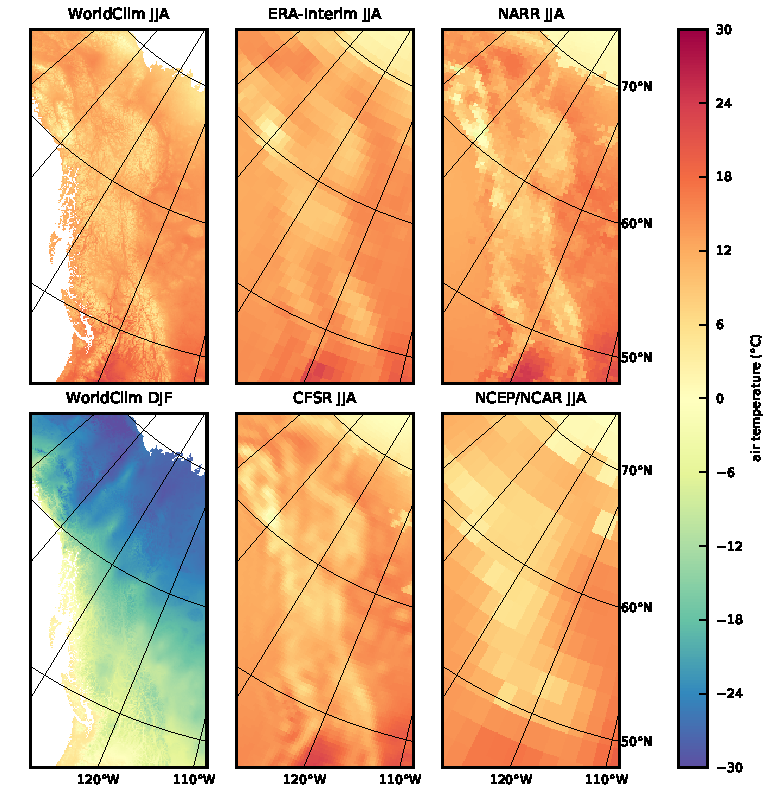
\includegraphics[width=13cm]{cordillera-climate-temp}
	\end{center}
	\caption{Summer temperature maps from the five datasets used in this study and winter temperature map from the WorldClim dataset.}
	\label{fig:temp}
\end{figure}

Figure~\ref{fig:temp} shows the spatial distribution of summer (JJA) air surface temperatures from the five climate datasets used in the study, and winter (DJF) air surface temperatures from the WorldClim interpolated observation data. Summer temperatures are most relevant to the glacier model as they drive summer melt.

As can be expected, temperatures decrease with latitude, and regions further inland experience colder winters. It should be noted that the temperature gradient is much stronger in the winter than it is in the summer, and that at low elevations, temperatures get well above zero during the summer months in the entire modelling domain. In other words, there is a strong seasonality contrast beween coastal and inland regions, and regions where mean annual temperatures are well below freezing do experience warm summers.

\begin{figure}[t]
	\vspace*{2mm}
	\begin{center}
		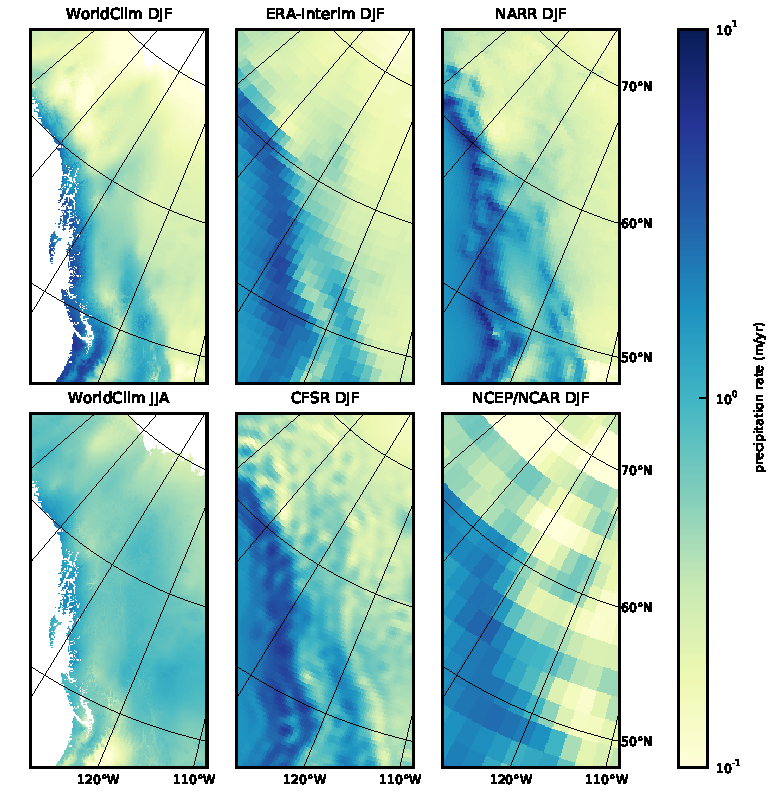
\includegraphics[width=13cm]{cordillera-climate-prec}
	\end{center}
	\caption{Winter precipitation rate maps from the five datasets used in this study and summer precipitation map from the WorldClim dataset.}
	\label{fig:prec}
\end{figure}

Figure~\ref{fig:prec} shows the spatial distribution of winter (DJF) precipitation rates from the five climate datasets used in the study, and summer (JJA) precipitation rates from the WorldClim interpolated observation data. Winter precipitation is most relevant to the glacier model as it drives winter accumulation.

Once again expectedly, coastal regions recieve much more precipitation than inland ones due to the unborken topographical barrier of the Boundary Ranges / Coast Mountains / Cascadia. It should be noted that from a glacier mass-balance view, this contrast is made even stronger by the difference of timing of the precipitation peak through the year. Although coastal regions experience most precipitation in the accumulation season, inland regions experience dry winters and most of the precipitation falls as rain during the summer months.

In regions like Northern Yukon and Alaska, dry winters and warm summers prevent snow accumulation and glacial inception despite of mean annual temperatures being well below zero at present. In order to account for these strong gradients in seasonality, we use monthly means to drive the ice sheet model. Previous runs made with mean annual temperature and precipitation forcing and not presented here lead to unrealistic ice cover in Northern Yukon and Alaska even under present-day climate while leaving the Coast Mountains free of ice.

% ----------------------------------------------------------------------

\subsection{Preprocessing and lapse-rate corrections}

Air surface temperature and precipitation rates from the NCEP/NCAR reanalysis, the ERA-Interim reanalysis, the CFSR, the NARR and WorldClim data were reprojected to Canadian Atlas Lambert (EPSG code XXXX\todo{add EPSG code}) conformal conic projection. The data were bilinearly interpolated to the model resolution of 10\,km, which is not shown by figures~\ref{fig:temp} and~\ref{fig:prec}.

For the WorldClim data, data holes in oceanic areas were filled by a nearest-neighbour extrapolation to allow ice to extend to these regions.

For the CFSR, an alternative forcing was prepared by smoothing the precipitation fields to avoid artifacts seen in figure~\ref{fig:prec}. This was done by averaging data locally in a circular neighbourhood of 7 pixels in diameter prior to reprojection. However the effect of smoothin the precipitation field is very limited as we will see further. All the preprocessing steps were made in GRASS~GIS using scripts made available on the first author's website.

\begin{figure}[t]
	\vspace*{2mm}
	\begin{center}
		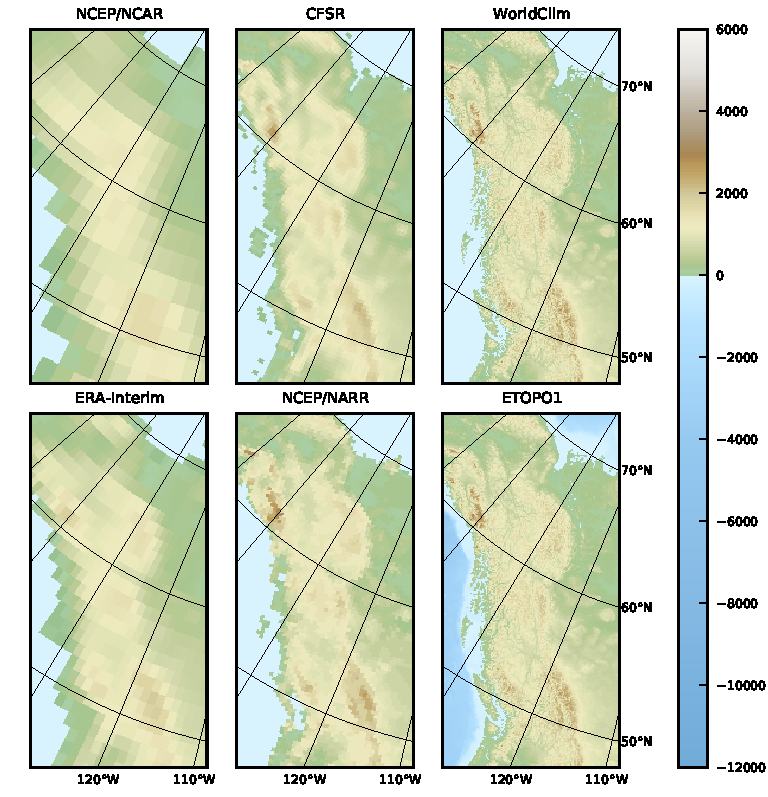
\includegraphics[width=13cm]{cordillera-climate-topo}
	\end{center}
	\caption{Reference topography used for temperature lapse-rate corrections from the five climate datasets used in the study and ETOPO1 topography used as basal condition for the ice flow model.}
	\label{fig:topo}
\end{figure}

Throughout the simulation, the numerical model dynamically applies temperature lapse-rate corrections that account for both differences between the climate reference topography and the ice flow model topography, and the thickness of overlying ice thickness. The reference topography from the five forcing datasets as well as the ETOPO1\citep{data:etopo1} topography used to force the ice flow model are shown in figure~\ref{fig:topo}. A lapse-rate of 6\unit{\degree C\,km^{-1}} was used in all simulations. No lapse-rate corrections are applied to precipitation rate.

